
\section{Central moment dispersion measures}\label{CentralM}
The central moment dispersion measures are defined as
\begin{equation}
    \CMDM^{(p)} = \left\| X - \mE[X] \right\|_p
    \label{cmdm1}
\end{equation}
where $\|\cdot\|_p = (\mE[|\cdot|^p])^{1/p}$ is the $L^p$-norm.
Note that $\CMDM^{(p)}$ is a genuine dispersion measure for any $p$.
In contrast to the tail, downside and below threshold measures, \CMDM\ are
symmetric. They do not provide an excess penalty to the downside
events.

For $p=1$ the \CMDM\ is equivalent to \MAD\ dispersion measure described in Sec.~\ref{S:mMAD}.

However, the most famous member of this family is for $p=2$, the standard deviation, \SD.
It is profoundly related to the 1952 Markowitz portfolio theory, \cite{Markowitz} and \cite{Markowitz2}.
In the original work, Markowitz had used the variance (the square of standard deviation) as a dispersion measure. Often the
variance based optimal portfolio strategies are called mean-variance, \MV.\footnote{Markowitz original terminology was E-V short
for expected rate of return vs. variance. These days, E-V terminology is rarely used, it was replaced by mean-variance, \MV.}
We will use the terminology {\it \MV-based optimal portfolio strategies} to designate portfolio strategies where variance is the dispersion measure.

Obviously, the \SD\ and \MV\ optimal portfolios are identical. Therefore, the \SD\ and \MV\
efficient frontiers are identical.\footnote{Two efficient frontiers are identical if and only if the composition of the portfolios
belonging to them are identical.} However, there are slight differences between the two measures.
Note that variance is not a genuine dispersion measure. It violates the positive homogeneity axiom. However, the formalism
of optimal portfolio strategies, outlined in Sec.~\ref{strategies}, holds. As we will see in the next two subsections,
the \SD\ and \MV\ optimization algorithms tend to be different.
\MV\ portfolio optimization is often described as a QP while \SD\ as an SOCP problem. However,
QP can be viewed as a special case of SOCP. In this sense the \SD\ and \MV\ optimal portfolio algorithms
could be regarded as similar.

Fundamental differences exist between the Sharpe type optimal portfolios.
The \SD-Sharpe ratio is the original Sharpe ratio introduced in 1966 by Sharpe in \cite{Sharpe1966} (see also \cite{Sharpe1994}).
For this reason, we will call \SD-Sharpe ratio simply as Sharpe ratio, preserving the original recognized terminology.
The \MV-Sharpe ratio is different than the Sharpe ratio. Therefore, Sharpe and \MV-Sharpe optimal portfolios are different.
However, since the \SD\ and \MV\ efficient frontiers are identical,
the \MV-Sharpe optimal portfolio belongs to the \SD\ efficient frontier and vice versa.

Similarly, the \SD\ and \MV\ optimal portfolios for the same risk-aversion factor value are different.
In fact, $\lambda_\SD$ (\SD-aversion factor) and $\lambda_\MV$ (\MV-aversion factor)
are two distinct parameterizations of the same efficient frontier.

The next two subsections present the \SD\ and \MV\ based optimal portfolio strategies algorithms separately.
We will point out along the way to the differences and similarities between the two approaches.
Overall, we prefer the \SD\ representation since it met all the scalability properties provided by a genuine
dispersion measure, especially for Sharpe optimal portfolios. However, the \MV\ representation is equally valid and
numerically robust.

\BackToContents


\subsection{SD-based optimization strategies}\label{S:SD}

\subsubsection{SD dispersion measure}

Standard deviation, \SD, is a special case, for $p=2$, of central momentum dispersion measure defined
in Eq.~(\ref{cmdm1}), \ie,
\begin{equation}
    \SD = \sqrt{\VAR(r)},
    \label{sd01}
\end{equation}
where $\VAR(r)$ is the variance of the rate of return. For a portfolio, defined by the set of weights $\{w_k\}_{k=1,\cdots,M}$,
Eq.~(\ref{sd01}) can be rewritten as
\begin{equation}
    \SD = \sqrt{w^T\cdot C\cdot w},
    \label{sd02}
\end{equation}
where $C$ is the covariance matrix between the portfolio components.
Although for direct computations either Eq.~(\ref{sd01}) or
Eq.~(\ref{sd0}) is sufficient, it is useful to mention the following alternative expression
\begin{equation}
    \SD = \| U\cdot w \|_2,
    \label{sd0}
\end{equation}
where $\|\cdot\|_2$ is the Euclidian norm and $U$ is a matrix such that $U^T\cdot U = C$. In general, $U$ is not unique.
If $C$ is a positive defined matrix, then $U$ can be given by the
Cholesky factorization. If $C$ is only positive semidefinite,\footnote{$C$ can be semidefinite if one of the portfolio components
is a risk-free asset (with zero volatility), \eg\ a pure cash position. \azapy\ implementation covers these cases too.} then $U$ can be computed as the
square root matrix.\footnote{The square root matrix of $C$ is the unique semidefinite matrix $U$ such that $U\cdot U = C$.}

\BackToContents


\subsubsection{SD optimal portfolio}
This optimization is described by Eqs.~(\ref{gg1}) from Sec~\ref{strategies} point~\ref{OptRisk},
where $\rho$ is given by \SD\ from Eq.\ (\ref{sd0}).
It is the following SOCP problem.

\bigskip
\noindent Minimize over $\{ \{w_k\}_{k=1,\cdots,M}, \eta \}$
\begin{subequations}\label{sd1}
\begin{align}
    & g = \eta, \label{sd1a} \\
    \st & \| U w \|_2 \leq \eta, \label{sd1b} \\
        & \sum_{k=1}^M w_k \mu_k \geq \mu_0, \label{sd1c} \\
        & \sum_{k=1}^K w_k = 1, \label{sd1d} \\
        & \eta \geq 0, \label{sd1f} \\
        & w_k \geq 0, \label{sd1e}
\end{align}
\end{subequations}

\noindent where $\mu$ from Eq.~(\ref{sd1c})
is the targeted portfolio rate of return, while $\mu_k$ for $k=1,\cdots,M$
are the portfolio components expected rate of returns.
Then, we have
\begin{subequations}\label{sd2}
\begin{align}
    \RR &= \sum_{k=1}^M w_k^* \mu_k, \label{sd2a} \\
    \SD &= g^*, \label{sd2b}
\end{align}
\end{subequations}

\noindent where $^*$ denotes the solution of SOCP problem.
In addition to the optimal portfolio weights $\{w_k^*\}_{k=1,\cdots,M}$ and expected
rate of return $\RR$, the
SOCP solution provides information about the portfolio standard deviation \SD.

\bigskip
\noindent Here is an example, using the \azapy\ package, of how to compute the \SD\ optimal portfolio.
The \SD\ time horizon was set to one quarter and the calibration is performed using 3.25 years of
close-adjusted historical prices (default settings).
For more details see the package documentation at \azapydoc.

\lstinputlisting[language=Python]{../PyScripts/SD_RiskOptim.py}

\BackToContents


\subsubsection{Minimum SD portfolio}

Following the results from Sec.~\ref{strategies} point~\ref{MinRisk},
the algorithm to compute the optimal portfolio with minimum \SD\ is given by the SOCP problem from Eqs.~(\ref{sd1}) where
$\mu$ from r.h.s. of Eq.~(\ref{sd1c}) is set to a value equal to the smallest expected rate of
return among the portfolio components, \ie\ $\mu=\min_k\{\mu_k\}$.

\bigskip
\noindent Here is an example, using the \azapy\ package, of how to compute the minimum \SD\ portfolio.
The \SD\ time horizon was set to one quarter and the calibration is performed using 3.25 years of
close-adjusted historical prices (default settings).
For more details see the package documentation at \azapydoc.

\lstinputlisting[language=Python]{../PyScripts/SD_MinRisk.py}

\BackToContents


\subsubsection{SD optimal portfolio for targeted risk value}
This optimization is described by Eqs.~(\ref{gg2}) from Sec.~\ref{strategies} point~\ref{TargetRisk},
where $\rho$ given by \SD\ from Eq.\ (\ref{sd0}).
It is the following SOCP problem.

\bigskip
\noindent Maximize over $\{ w_k \}_{k=1,\cdots, M}$
\begin{subequations}\label{sd3}
\begin{align}
    & g = \sum_{k=1}^M w_k \mu_k, \label{sd3a} \\
    \st & \| U w\|_2 \leq \SD_0, \label{sd3b} \\
        & \sum_{k=1}^M w_k = 1, \label{sd3c} \\
        & w_k \geq 0, \label{sd3d}
\end{align}
\end{subequations}

\noindent where $\SD_0$ from Eq.~(\ref{sd3b}) is the targeted portfolio \SD\ value.
The portfolio expected rate of return is given by the optimal value of the objective
function, \ie,
\begin{equation}
    \RR = g^*, \label{sd4}
\end{equation}

\noindent and the optimal portfolio weights by $\{w^*_k\}_{k=1,\cdots,M}$. The superscript $^*$ denotes the
solution of SOCP problem.


\bigskip
\noindent Here is an example, using the \azapy\ package, of how to compute the optimal portfolio
with the same \SD\ as the equal weighted portfolio.
The \SD\ time horizon was set to one quarter and the calibration is performed using 3.25 years of
close-adjusted historical prices (default settings).
For more details see the package documentation at \azapydoc.

\lstinputlisting[language=Python]{../PyScripts/SD_InvNrisk.py}

\BackToContents


\subsubsection{SD optimal portfolio for fixed risk-aversion factor}
This optimization is described by Eqs.~(\ref{gg3}) from Sec.~\ref{strategies} point~\ref{RiskAverse},
where $\rho$ is given by \SD\ from Eq.\ (\ref{sd0}).
It is the following SOCP problem.

\bigskip
\noindent Maximize over $\{ \{w_k\}_{k=1,\cdots,M}, \eta \}$
\begin{subequations}\label{sd5}
\begin{align}
    & g = \sum_{k=1}^M w_k \mu_k -\lambda \eta, \label{sd5a} \\
    \st & \| U w\|_2 \leq \eta, \label{sd5b} \\
        & \sum_{k=1}^m w_k = 1, \label{sd5c} \\
        & \eta \geq 0, \label{sd5e} \\
        & w_k \geq 0, \label{sd5d}
\end{align}
\end{subequations}

\noindent where $\lambda$ from Eq.~(\ref{sd5a}) is the risk-aversion factor.
Then, we have
\begin{subequations}\label{sd6}
\begin{align}
    \RR &= \sum_{k=1}^M w_k^* \mu_k, \label{sd6a} \\
    \SD &= \eta^*, \label{sd6b}
\end{align}
\end{subequations}

\noindent where $^*$ denotes the solution of SOCP problem.
In addition to the optimal portfolio weights $\{w_k^*\}_{k=1,\cdots,M}$ and expected rate of return $\RR$, the
SOCP solution provides information about the portfolio \SD.

\bigskip
\noindent Here is an example, using the \azapy\ package, of how to compute the optimal portfolio
for a given value of the risk-aversion factor $\lambda$.
The \SD\ time horizon was set to one quarter and the calibration is performed using 3.25 years of
close-adjusted historical prices (default settings).
For more details see the package documentation at \azapydoc.

\lstinputlisting[language=Python]{../PyScripts/SD_Averse.py}

\BackToContents


\subsubsection{Sharpe optimal portfolio - maximization solution}
This optimization targets the maximization of Sharpe ratio. It is based on
Eqs.~(\ref{gg4}) from Sec.~\ref{strategies} point~\ref{MaxSharpe},
where $\rho$ is given by \SD\ from Eq.~(\ref{sd0}).
The optimization can be formulated as an SOCP problem
if Eq.~(\ref{gg4b}) can be expressed as a second order cone constraint.  This can be achieved by
introducing the variable transformations $\bw_k = t w_k$. Then, the SOCP
problem can be written as follows.

\bigskip
\noindent Maximize over $\{ \{\bw_k\}_{k=1,\cdots,M}, t\}$
\begin{subequations}\label{sd7}
\begin{align}
    & g = \sum_{k=1}^M \bw_k \mu_k - \mu_0 t, \label{sd7a} \\
    \st & \| U \bw \|_2 \leq 1, \label{sd7b} \\
        & \sum_{k=1}^M \bw_k - t = 0, \label{sd7c} \\
        & t \geq 0, \label{sd7e} \\
        & \bw_k \geq 0, \label{sd7d}
\end{align}
\end{subequations}

\noindent where $\mu_0$ from Eq.~(\ref{sd7a}) is the risk-free rate accessible to the investor.
Then, we have
\begin{subequations}\label{sd8}
\begin{align}
    w_k &= \frac{\bw_k^*}{t^*}, \label{sd8a} \\
    \RR &= \frac{g^*}{t^*} + \mu_0, \label{sd8c} \\
    \Sharpe &= g^*, \label{sd8b} \\
    \SD &= \frac{1}{t^*}, \label{sd8d}
\end{align}
\end{subequations}

\noindent where $^*$ denotes the solution of SOCP problem.
In addition to the optimal portfolio weights $\{w_k\}_{k=1,\cdots,M}$, expected rate of return $\RR$ and
the Sharpe ratio $\Sharpe$,
the SOCP solution provides information about the portfolio \SD.


\bigskip
\noindent Here is an example, using the \azapy\ package, of how to compute the Sharpe optimal portfolio using the maximization
of Sharpe ratio.
The \SD\ time horizon was set to one quarter and the calibration is performed using 3.25 years of
close-adjusted historical prices (default settings).
For more details see the package documentation at \azapydoc.

\lstinputlisting[language=Python]{../PyScripts/SD_Sharpe.py}

\BackToContents


\subsubsection{Sharpe optimal portfolio - minimization solution}
This optimization targets the minimization of the inverse of Sharpe ratio.
It is  described by Eqs.~(\ref{gg8}) from Sec.~\ref{strategies} point~\ref{MinSharpe}, where
$\rho$ is given by \SD\ from Eq.~(\ref{sd0}).
The optimization can be formulated as an SOCP problem if Eq.~(\ref{gg8a}) can be expressed as second order cone constraint. This can be achieved by
introducing the  variable transformations
$\bw_k = t w_k$ and $\bbeta = t\eta$.
Then, the SOCP problem can be written as follows.

\bigskip
\noindent Minimize over $\{ \{ \bw_k \}_{k=1,\cdots,M}, \bbeta, t \}$
\begin{subequations}\label{sd9}
\begin{align}
    & g = \bbeta, \label{sd9a} \\
    \st & \| U \bw \|_2 \leq \bbeta, \label{sd9b} \\
        & \sum_{k=1}^M \bw_k \mu_k - \mu_0 t = 1, \label{sd9c} \\
        & \sum_{k=1}^M \bw_k - t = 0, \label{sd9d} \\
        & t \geq 0, \label{sd9f} \\
        & \bbeta \geq 0, \label{sd9g} \\
        & \bw_k \geq 0, \label{sd9e}
\end{align}
\end{subequations}

\noindent where $\mu_0$ from Eq.~(\ref{sd9c}) is the risk-free rate accessible to the investor.
Then, we have
\begin{subequations}\label{sd10}
\begin{align}
    w_k &= \frac{\bw_k^*}{t^*}, \label{sd10a} \\
    \RR &= \frac{1}{t^*} + \mu_0, \label{sd10c} \\
    \Sharpe &= \frac{1}{g^*}, \label{sd10b} \\
    \SD &= \frac{g^*}{t^*}, \label{sd10d}
\end{align}
\end{subequations}

\noindent where $^*$ denotes the solution of SOCP problem.
In addition to the optimal portfolio weights $\{w_k\}_{k=1,\cdots,M}$, expected rate of return $\RR$ and
Sharpe ratio $\Sharpe$,
the SOCP solution provides information about the portfolio \SD.

\bigskip
\noindent Here is an example, using the \azapy\ package, of how to compute the Sharpe optimal portfolio using the minimization
of the inverse of Sharpe ratio.
The \SD\ time horizon was set to one quarter and the calibration is performed using 3.25 years of
close-adjusted historical prices (default settings).
For more details see the package documentation at \azapydoc.

\lstinputlisting[language=Python]{../PyScripts/SD_InvSharpe.py}

\BackToContents

\subsubsection{SD frontiers}

Here is an example of how to compute the \SD\ frontiers using the \azapy\
package. The \SD\ time horizon was set to one quarter and the calibration is performed using 3.25 years of
close-adjusted historical prices (default settings).
For more details see the package documentation at \azapydoc.

The script produces the plots in Figs. \ref{SD_fig1a} and \ref{SD_fig1b}
for historical data collected up to 2021-07-27.

\lstinputlisting[language=Python]{../PyScripts/SD_frontiers.py}

\begin{figure}[H]
\centering
\begin{subfigure}{.5\textwidth}
  \centering
  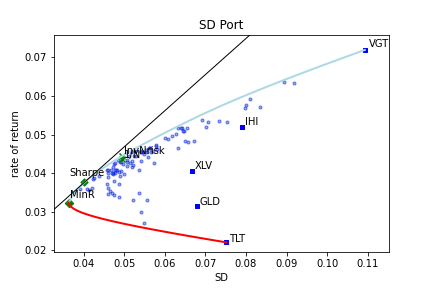
\includegraphics[width=.95\linewidth]{../figs/SDFrontier1.png}
  \caption{Rate of return vs. \SD}
  \label{SD_fig1a}
\end{subfigure}%
\begin{subfigure}{.5\textwidth}
  \centering
  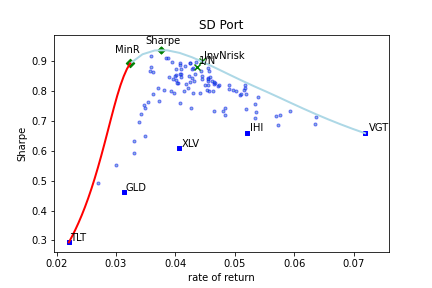
\includegraphics[width=.95\linewidth]{../figs/SDFrontier2.png}
  \caption{Sharpe vs. rate of return}
  \label{SD_fig1b}
\end{subfigure}
\caption{\SD\ frontiers.}
\label{SD_fig1}
\end{figure}

\BackToContents

\subsubsection{Backtesting Sharpe optimal portfolio}

Here is an example, using \azapy\ package, of computing a portfolio backtesting.
For this example, we have chosen a portfolio quarterly rebalanced according
to the maximization of Sharpe ratio. At each rebalancing date,
the portfolio weights
are calibrated based on 3.25 years of prior historical market data.

Other rebalancing strategies can be considered
by changing the value of {\it rtype} parameter in the call of {\it set\_model} function below.
For more details see the package documentation at \azapydoc.

\lstinputlisting[language=Python]{../PyScripts/SD_Port.py}

\begin{figure}[H]
    \centering
    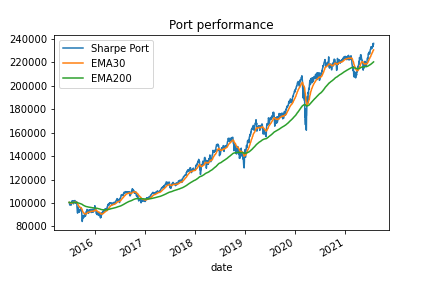
\includegraphics[width=.95\linewidth]{../figs/Port_SD_Sharpe.png}
    \caption{Backtesting of quarterly rebalanced Sharpe optimal portfolio.}
    \label{SD_Port_fig}
\end{figure}

\BackToContents



\subsection{MV-based optimization strategies}\label{S:MV}

\subsubsection{MV dispersion measure}
Variance is the dispersion measure for \MV-based optimal portfolios.
For a portfolio defined by the vector of weights $w$, the variance can
be expressed as
\begin{equation}
    \VAR = w^T \cdot C \cdot w,
    \label{mv00}
\end{equation}
where $C$ is the covariance matrix between the portfolio components.
Alternatively, assuming $C=U^T\cdot U$ factorization, \VAR\ can be rewritten in terms of Euclidian norm as
\begin{equation}
    \VAR = \|U \cdot w\|_2^2.
    \label{mv0}
\end{equation}
We will use both expressions.

\BackToContents

\subsubsection{MV optimal portfolio}
This optimization is described by Eqs.~(\ref{gg1}) from Sec~\ref{strategies} point~\ref{OptRisk},
where $\rho$ is given by \VAR\ from Eq.~(\ref{mv00}).
It is the following QP problem.

\bigskip
\noindent Minimize over $\{ \{w_k\}_{k=1,\cdots,M}, t\}$
\begin{subequations}\label{mv1}
\begin{align}
    & g = \frac{1}{2} w^T C w, \label{mv1a} \\
    \st & \sum_{k=1}^M w_k \mu_k \geq \mu_0, \label{mv1b} \\
        & \sum_{k=1}^M w_k = 1, \label{mv1c} \\
        & w_k \geq 0, \label{mv1d}
\end{align}
\end{subequations}

\noindent where $\mu$, in Eq.~(\ref{mv1b}),
is the targeted portfolio expected rate of return, while $\mu_k$ for $k=1,\cdots,M$
are the portfolio components expected rate of returns.
Then, we have
\begin{subequations}\label{mv2}
\begin{align}
    \RR &= \sum_{k=1}^M w_k^* \mu_k, \label{mv2a} \\
    \VAR &= 2 g^*, \label{mv2b}
\end{align}
\end{subequations}

\noindent where $^*$ denotes the solution of QP problem.
In addition to the optimal portfolio weights $\{w_k^*\}_{k=1,\cdots,M}$ and expected
rate of return $\RR$, the
QP solution provides information about the portfolio \VAR.

The set of equations~(\ref{mv1}) are the most celebrated and the most printed set of equations in the world of portfolio optimizations.
They are at the core of Markowitz pioneer work of portfolio theory \cite{Markowitz} and \cite{Markowitz2}. Up to the customary $1/2$ factor
the solution of Eqs.~(\ref{mv1}) is the same as the solution of Eqs.~(\ref{sd1}). In fact, they illustrate the generic transformation of
a QP into an SOCP problem.

\bigskip
\noindent Here is an example, using the \azapy\ package, of how to compute the \MV\ optimal portfolio.
The \VAR\ time horizon was set to one quarter and the calibration is performed using 3.25 years of
close-adjusted historical prices (default settings).
For more details see the package documentation at \azapydoc.

\lstinputlisting[language=Python]{../PyScripts/MV_RiskOptim.py}

\BackToContents


\subsubsection{Minimum \VAR\ portfolio}

Following the results from Sec.~\ref{strategies} point~\ref{MinRisk},
the algorithm to compute the portfolio with minimum \VAR\ is given by the QP problem from Eqs.~(\ref{mv1}) where
$\mu$ from r.h.s. of Eq.~(\ref{mv1b}) is set to a value equal to the smallest expected rate of
return among the portfolio components, \ie\ $\mu=\min_k\{\mu_k\}$.
Note that minimum \VAR\ and minimum \SD\ portfolios are identical.

\bigskip
\noindent Here is an example, using the \azapy\ package, of how to compute the minimum \VAR\ optimal portfolio.
The \VAR\ time horizon was set to one quarter and the calibration is performed using 3.25 years of
close-adjusted historical prices (default settings).
For more details see the package documentation at \azapydoc.

\lstinputlisting[language=Python]{../PyScripts/MV_MinRisk.py}

\BackToContents


\subsubsection{MV optimal portfolio for targeted risk value}
This optimization is described by Eqs.~(\ref{gg2}) from Sec.~\ref{strategies} point~\ref{TargetRisk},
where $\rho$ given by \VAR\ from Eq.\ (\ref{mv0}).
It is the following SOCP problem.

\bigskip
\noindent Maximize over $\{ w_k \}_{k=1,\cdots, M}$
\begin{subequations}\label{mv3}
\begin{align}
    & g = \sum_{k=1}^M w_k \mu_k, \label{mv3a} \\
    \st & \| U w\|_2 \leq \sqrt{\VAR_0}, \label{mv3b} \\
        & \sum_{k=1}^M w_k = 1, \label{mv3c} \\
        & w_k \geq 0, \label{mv3d}
\end{align}
\end{subequations}

\noindent where $\VAR_0$ from Eq.~(\ref{mv3b}) is the targeted portfolio variance value.
The portfolio expected rate of return is given by the value of the objective
function, \ie,
\begin{equation}
    \RR = g^*, \label{mv4}
\end{equation}

\noindent and the optimal portfolio weights by $\{w^*_k\}_{k=1,\cdots,M}$. The superscript $^*$ denotes the
solution of SOCP problem.

By and large, these sets of equations are a reprint of Eqs.~(\ref{sd3}) and (\ref{sd4}).
Therefore, the \MV\ and \SD\ optimal portfolios with similar targeted risk (\ie\ $\VAR_0 = \SD_0^2$) are identical.

\bigskip
\noindent Here is an example, using the \azapy\ package, of how to compute the optimal portfolio
with the same \VAR\ as the equal weighted portfolio.
The \VAR\ time horizon was set to one quarter and the calibration is performed using 3.25 years of
close-adjusted historical prices (default settings).
For more details see the package documentation at \azapydoc.

\lstinputlisting[language=Python]{../PyScripts/MV_InvNrisk.py}

\BackToContents


\subsubsection{MV optimal portfolio for fixed risk-aversion factor}
This optimization is described by Eqs.~(\ref{gg3}) from Sec.~\ref{strategies} point~\ref{RiskAverse},
where $\rho$ is given by \VAR\ from Eq.\ (\ref{mv00}).
It can be written as the following QP problem.

\bigskip
\noindent Minimize over $\{ w_k \}_{k=1,\cdots,M}$
\begin{subequations}\label{mv5}
\begin{align}
    & g = \frac{1}{2}\left( w^T C w \right) - \frac{1}{2\lambda} \sum_{k=1}^M w_k \mu_k, \label{mv5a} \\
    \st & \sum_{k=1}^M w_k =1, \label{mv5b} \\
        & w_k \geq 0, \label{mv5c}
\end{align}
\end{subequations}

\noindent where $\lambda$ from Eq.\ (\ref{mv5a}) is the risk-aversion factor.
Then, we have
\begin{subequations}\label{mv6}
\begin{align}
    \RR &= \sum_{k=1}^M w_k^* \mu_k, \label{mv6a} \\
    \VAR &= 2 g^* + \frac{\RR}{\lambda}, \label{mv6b}
\end{align}
\end{subequations}

\noindent where $^*$ denotes the solution of QP problem.
In addition to the optimal portfolio weights $\{w_k^*\}_{k=1,\cdots,M}$ and expected rate of return $\RR$, the
QP solution provides information about the portfolio \VAR.

Note that, in this case, the \SD\ and \MV\ optimal portfolio for the same value of $\lambda$ are different.
Both portfolios belong to the \MV\ efficient frontiers (identical with \SD\ efficient frontiers). However, $\lambda$
in the \MV\ representation provides a different parametrization of the efficient frontiers than $\lambda$ in the
\SD\ representation.

\bigskip
\noindent Here is an example, using the \azapy\ package, of how to compute the optimal portfolio
for a given value of the risk-aversion factor $\lambda$.
The \VAR\ time horizon was set to one quarter and the calibration is performed using 3.25 years of
close-adjusted historical prices (default settings).
For more details see the package documentation at \azapydoc.

\lstinputlisting[language=Python]{../PyScripts/MV_Averse.py}

\BackToContents


\subsubsection{\MV-Sharpe optimal portfolio - maximization solution}
This optimization targets the maximization of \MV-Sharpe ratio. It is based on
Eqs.~(\ref{gg4}) from Sec.~\ref{strategies} point~\ref{MaxSharpe},
where $\rho$ is given by \VAR\ from Eq.~(\ref{mv00}).
The optimization can be formulated as an SOCP problem
if Eq.~(\ref{gg4b}) can be expressed as a second order cone constraint.
This can be achieved by
introducing the variable transformations
$\bw_k = t w_k$. Then, the SOCP problem can be written as follows.

\bigskip
\noindent Maximize over $\{ \{ \bw_k\}_{k=1,\cdots,M}, t\}$
\begin{subequations}\label{mv7}
\begin{align}
    & g = \sum_{k=1}^M \bw_k \mu_k - \mu_0 t, \label{mv7a} \\
    \st & \left\| \left(\bw^T \cdot U^T , t - \frac{1}{4} \right)^T \right\|_2 \leq t + \frac{1}{4}, \label{mv7b} \\
        & \sum_{k=1}^M \bw_k - t = 0, \label{mv7c} \\
        & t \geq 0, \label{mv7e} \\
        & w_k \geq 0, \label{mv7d}
\end{align}
\end{subequations}

\noindent where $\mu_0$ from Eq.~(\ref{sd7a}) is the risk-free rate accessible to the investor.

Equation~(\ref{mv7b}) is the Euclidian norm representation of
\begin{equation}
    \bw^T \cdot C \cdot \bw \leq t,
    \label{mv8}
\end{equation}
originated from Eq.~(\ref{gg6b}) after a multiplication by $t$ on both sides. Indeed, it is straightforward to show
that, Eq.~(\ref{mv8}) is equivalent to
\begin{equation}
    \left[ \bw^T C \bw +\left(t - \frac{1}{4}\right)^2 \right]^{1/2} \leq t + \frac{1}{4}.
    \label{mv9}
\end{equation}
The l.h.s. is the Euclidian norm of $\left(\bw^T \cdot U^T , t - \frac{1}{4} \right)^T$ vector, that enters
in Eq.~(\ref{mv7b}).


Then, we have
\begin{subequations}\label{mv10}
\begin{align}
    w_k &= \frac{\bw_k^*}{t^*} , \label{mv10a} \\
    \Sharpe &= g^*, \label{mv10b} \\
    \RR &= \frac{g^*}{t^*} + \mu_0, \label{mv10c} \\
    \VAR &= \frac{1}{t^*}, \label{mv10d}
\end{align}
\end{subequations}

\noindent where $^*$ denotes the solution of SOCP problem.
In addition to the optimal portfolio weights $\{w_k\}_{k=1,\cdots,M}$, expected rate of return $\RR$ and
the \MV-Sharpe ratio $\Sharpe$,
the SOCP solution provides information about the portfolio \VAR.


\bigskip
\noindent Here is an example, using the \azapy\ package, of how to compute the \MV-Sharpe optimal portfolio using the maximization
of \MV-Sharpe ratio.
The \VAR\ time horizon was set to one quarter and the calibration is performed using 3.25 years of
close-adjusted historical prices (default settings).
For more details see the package documentation at \azapydoc.

\lstinputlisting[language=Python]{../PyScripts/MV_Sharpe.py}

\BackToContents

\subsubsection{\MV-Sharpe optimal portfolio - minimization solution}
This optimization targets the minimization of the inverse of \MV-Sharpe ratio.
It is described by Eqs.~(\ref{gg8}) from Sec.~\ref{strategies} point~\ref{MinSharpe}, where
$\rho$ is given by \VAR\ from Eq.~(\ref{mv0}).
The optimization can be formulated as an SOCP problem if Eq.~(\ref{gg8a}) can be expressed as a second order cone constraint. This can be achieved by
introducing a new variable $\eta$ such that
\begin{equation}
    \eta \geq t w^T \cdot C \cdot w,
    \label{mv11}
\end{equation}
and the variable transformations $\bw_k = t w_k$.
Then, the SOCP problem can be written as follows.

\bigskip
\noindent Minimize over $\{ \{ \bw_k\}_{k=1,\cdots,M}, \eta, t\}$
\begin{subequations}\label{mv12}
\begin{align}
    & g = \eta, \label{mv12a} \\
    \st & \left\| \left( \bw^T \cdot U^T , \frac{\eta}{\sqrt{2}} , \frac{t}{\sqrt{2}}  \right)^T \right\|_2
                \leq \frac{\eta}{\sqrt{2}}  + \frac{t}{\sqrt{2}} , \label{mv12b} \\
        & \sum_{k=1}^m \bw_k \mu_k - \mu_0 t = 1, \label{mv12c} \\
        & \sum_{k=1}^M \bw_k - t = 0, \label{mv12d} \\
        &t \geq 0, \label{mv12e} \\
        &\eta \geq 0, \label{mv12f} \\
        &\bw_k \geq 0, \label{mv12g}
 \end{align}
\end{subequations}

\noindent where $\mu_0$ from Eq.~(\ref{mv12c}) is the risk-free rate accessible to the investor.

Equation~(\ref{mv12b}) is the Euclidian norm representation of Eq.~(\ref{mv11}), after
an additional multiplication by $t$ on both sides, \ie,
\begin{equation}
    \bw^T\cdot C\cdot \bw \leq t\eta.
    \label{mv13}
\end{equation}
Indeed, it is straightforward to show that, Eq.~(\ref{mv13}) is equivalent to
\begin{equation}
    \left( \bw^T C \bw + \frac{1}{2}\eta^2 + \frac{1}{2}t^2 \right)^{1/2} \leq \frac{\eta}{\sqrt{2}} + \frac{t}{\sqrt{2}}.
    \label{mv14}
\end{equation}
The l.h.s. is the Euclidian norm of $\left( \bw^T \cdot U^T , \frac{\eta}{\sqrt{2}} , \frac{t}{\sqrt{2}}  \right)^T$ vector, that
enters in Eq.~(\ref{mv12b}).

Then, we have
\begin{subequations}\label{mv15}
\begin{align}
    w_k &= \frac{\bw_k^*}{t^*}, \label{mv15a} \\
    \RR &= \frac{1}{t^*} + \mu_0, \label{mv15c} \\
    \Sharpe &= \frac{1}{g^*}, \label{mv15b} \\
    \VAR &= \frac{g^*}{t^*}, \label{mv15d}
 \end{align}
\end{subequations}

\noindent where $^*$ denotes the solution of SOCP problem.
In addition to the optimal portfolio weights $\{w_k\}_{k=1,\cdots,M}$, expected rate of return $\RR$ and
the \MV-Sharpe ratio $\Sharpe$,
the SOCP solution provides information about the portfolio \VAR.

\bigskip
\noindent Here is an example, using the \azapy\ package, of how to compute the \MV-Sharpe optimal portfolio using the minimization
of the inverse of \MV-Sharpe ratio.
The \VAR\ time horizon was set to one quarter and the calibration is performed using 3.25 years of
close-adjusted historical prices (default settings).
For more details see the package documentation at \azapydoc.

\lstinputlisting[language=Python]{../PyScripts/MV_InvSharpe.py}

\BackToContents


\subsubsection{MV frontiers}

Here is an example of how to compute the \MV\ frontiers using the \azapy\
package. The \VAR\ time horizon was set to one quarter and the calibration is performed using 3.25 years of
close-adjusted historical prices (default settings).
For more details see the package documentation at \azapydoc.

The script produces the plots in Figs. \ref{MV_fig1a} and \ref{MV_fig1b}
for historical data collected up to 2021-07-27.

\lstinputlisting[language=Python]{../PyScripts/MV_frontiers.py}

\begin{figure}[H]
\centering
\begin{subfigure}{.5\textwidth}
  \centering
  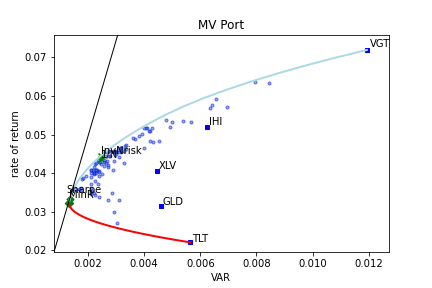
\includegraphics[width=.95\linewidth]{../figs/MVFrontier1.png}
  \caption{Rate of return vs. \VAR}
  \label{MV_fig1a}
\end{subfigure}%
\begin{subfigure}{.5\textwidth}
  \centering
  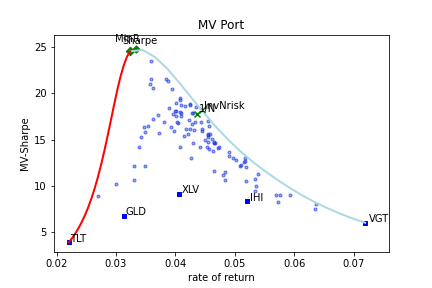
\includegraphics[width=.95\linewidth]{../figs/MVFrontier2.png}
  \caption{\MV-Sharpe vs. rate of return}
  \label{MV_fig1b}
\end{subfigure}
\caption{\MV\ frontiers.}
\label{MV_fig1}
\end{figure}

\BackToContents


\subsubsection{Backtesting MV-Sharpe optimal portfolio}

Here is an example, using \azapy\ package, of computing a portfolio backtesting.
For this example, we have chosen a portfolio quarterly rebalanced according
to the maximization of \MV-Sharpe ratio. At each rebalancing date,
the portfolio weights
are calibrated based on 3.25 years of prior historical market data.

Other rebalancing strategies can be considered
by changing the value of {\it rtype} parameter in the call of {\it set\_model} function below.
For more details see the package documentation at \azapydoc.

\lstinputlisting[language=Python]{../PyScripts/MV_Port.py}

\begin{figure}[H]
    \centering
    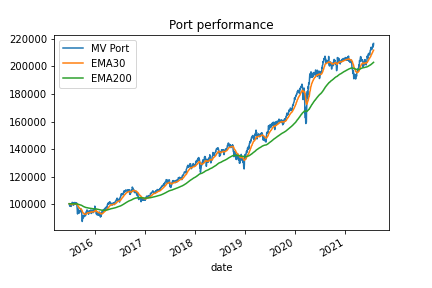
\includegraphics[width=.95\linewidth]{../figs/Port_MV_Sharpe.png}
    \caption{Backtesting of quarterly rebalanced \MV-Sharpe optimal portfolio.}
    \label{MV_Port_fig}
\end{figure}

\BackToContents



